\chapter{Purpose of the Application}
\setlength{\parskip}{1em}
The purpose of this application is to allow a user to ask for various information about games via voice commands. The user can ask many different things such as general information about the game, locations from the game as well as the different characters in the game itself. This is all done using Alexa and voice commands. For example if the user asks "what is Fallout?" Alexa will respond with information about Fallout as well as display a picture from the game. Similarly if the user asks "what is megaton?" Alexa will then respond with information about the location (Megaton) from the fallout franchise.

\begin{figure}[h!]
  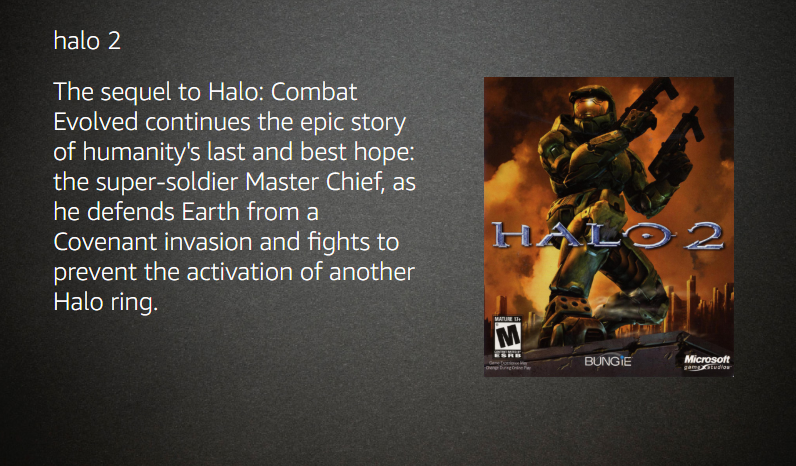
\includegraphics[width=\linewidth]{halo2.PNG}
  \caption{Game Intent}
  \label{fig:gameintent}
\end{figure}

This skill-set was made using the Giant Bomb API. Giant Bomb is a a gaming website which contains gaming related news, reviews and previews. In 2008 giant bomb created a wiki styled database to contain all the information available in the API such as characters, locations and general game knowledge. We used this API to help us create the app. 

A big part of the project was to gain better insight into how exactly gesture controls are created and what kind of gestures we should use for our given project. 
